\section{Efficiency Analysis}

Here we try to analyze the speedup of Parareal analytically, and then through
scalability studies conducted on the supercomputer Prince, here at NYU. 

\subsection{Theoretical Results}

We try to directly estimate the speedup of the Naive OpenMP implementation. We
denote our speedup $S$ by: (\cite{fieldstalk} slide 17)
\begin{equation*}
  S = \frac{\text{Time taken by fine solver}}{\text{Parareal time}}
\end{equation*}
Let the time taken by the fine and coarse solvers respectively be denoted by
$T_f$ and $T_g$. Furthermore, suppose we have the optimal amount of processors
$P$, such that $\Delta t = T/P$, where $T$ is the time to integrate up to.

Considering this, each step parareal makes a predictor and corrector
computation. The predictor is just a run of the coarse solver, costing $PT_g$.
The corrector has two parts, the fine and coarse portion. The fine portion is
parallelized optimally, and therefore costs just $T_f$, instead of $PT_f$.  In
addition, the coarse portion of the corrector takes advantage of the
\textit{first same as last} property, and doesn't have to be counted sepreately.
Recall, also, before the parareal iteration, we make an initial guess using one
coarse solve, $PT_g$. Therefore, for a parareal with $k$ iterations it would
have speedup:
\[
  S = \frac{PT_f}{PT_g + k(PT_g + T_f)} 
  = \frac{1}{\frac{T_g}{T_f} + k(\frac{T_g}{T_f} + \frac{1}{P})} 
  = \frac{1}{\frac{T_g}{T_f}(1+k) + \frac{k}{P}} 
\]
Notice, under the limit:
\[
  \lim_{P \to \infty} S = \frac{1}{\frac{T_g}{T_f}(1+k)} = \frac{T_f}{T_g(1+k)}
\]
Supposing we have the idealized case of $k = 1$, then we would find that this
would result in speedup $\frac{T_f}{2T_g}$, which, given that $T_g << T_f$,
could be significant. However, in practice, $k$ has to be taken to be large
enough so that $S$ isn't too great. This is one of the first indicators we have
of why $T_g << T_f$ must be true. 

\subsection{Scalability}

Since this algorithm is designed to take our numerical ODE techniques to a high
performance computing context, we would like to perform the standard scalability
tests using this algorithm, measuring how it scales to massively parallel
hardware.

All tests are performed on a single Prince node, having requested 28 processors.
We would be worried about other processes running on this node if this problem
was memory bound, however since the fine computation is performed in place and
the coarse operator has few points, the computation is compute bound.

\subsubsection{Strong Scaling Study}

A strong scaling study consists of fixing a total problem size, and increasing
the number of processors necessary. See figure \ref{fig:strong_scaling} for our
performed analysis.
\begin{figure}[!htb]
  \centering
  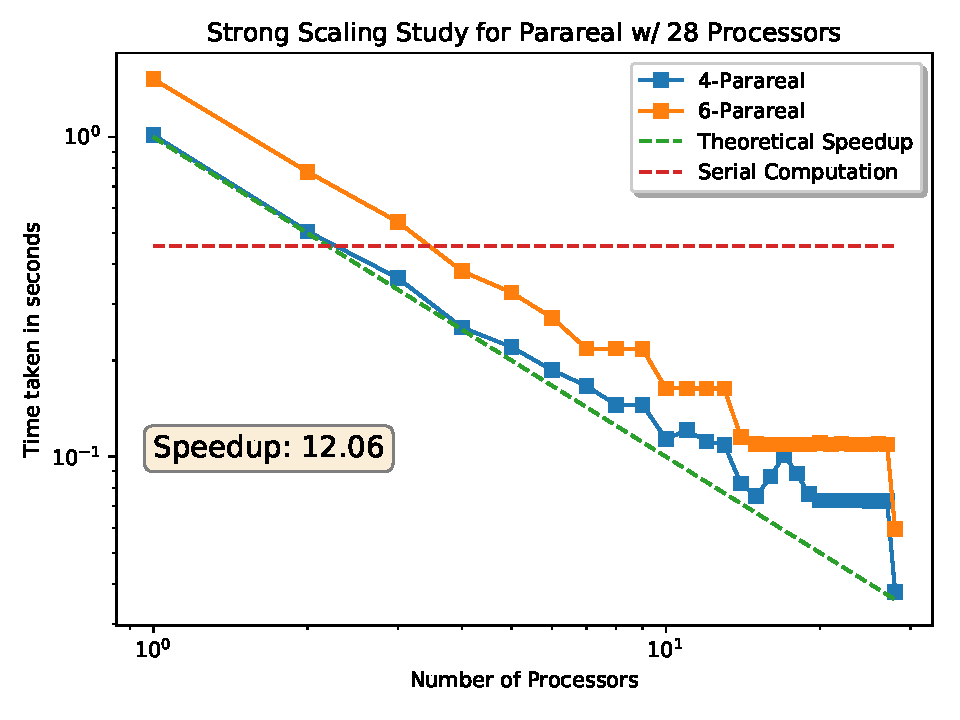
\includegraphics[width=.8\textwidth]{./resources/strong_scaling}
  \caption{This is a strong scaling study performed on the ODE $u' = u, u(0) =
  1$ integrating on time scale $[0, 4]$. Here we divided our time scale into
  pieces of size $4/P$, and then ran Parareal restricting the number of
  processors. Notice how the time taken doesn't improve from $14 \to
  28$.}\label{fig:strong_scaling}
\end{figure}
Note that figure \ref{fig:strong_scaling} presents a very interesting, and
dismal, phenomena. Notice how from processors $14 \to 27$ the speedup recieved
is negligable from the previous. Why does this occur? Recall that the optimal
number of processors for parareal iteration is the number of coarse steps, so
that we can process all of the $\fine$ integrators in one step. However,
supposing we have one less than optimal, the entire compute time is bounded by
that one thread that has to process two $\fine$ integrators. This is
troublesome.
In fact, suppose we desire to cut our time domain $[0, T]$ into $2N$ pieces.
Then any computation with number of processors $P$ taking value $N \to 2N-1$
will have the same computation time, theoretically.

Notice, however, that the general speedup does follow the theoretical linear
speedup we hope to see with $P$ processors, which is great.

\subsubsection{Weak Scaling Study}

The weak scaling study examines how the runtime increases as we increase the
amount of processors, working on a similar sized problem. See figure
\ref{fig:weak_scaling} for the results.
\begin{figure}[!htb]
  \centering
  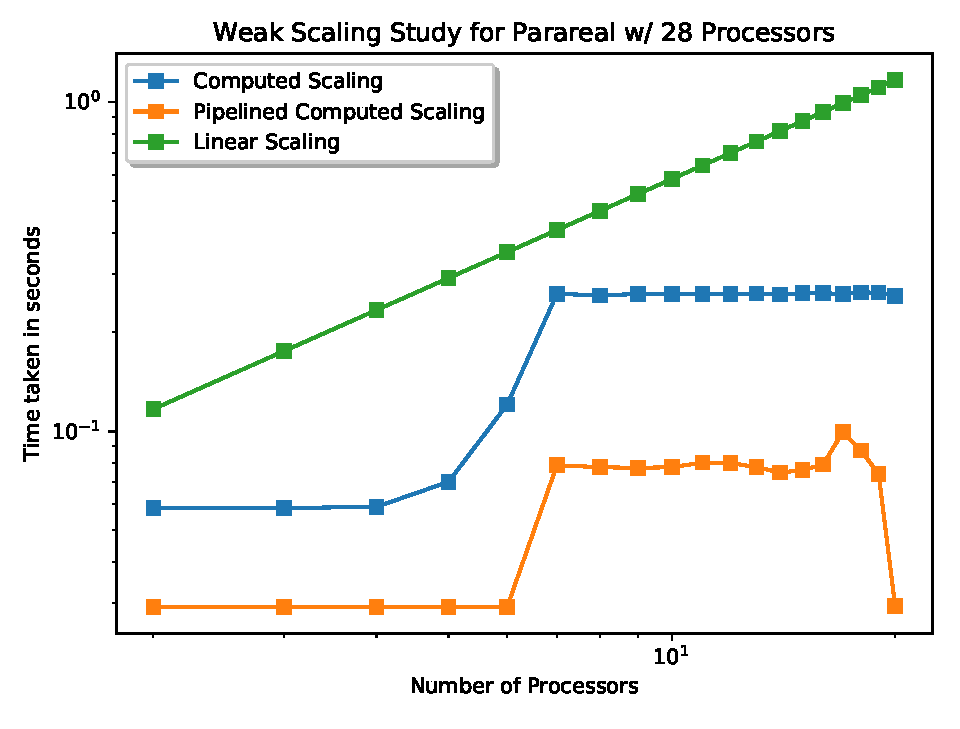
\includegraphics[width=.8\textwidth]{./resources/weak_scaling}
  \caption{}\label{fig:weak_scaling}
\end{figure}
We see that the Weak Scaling of parareal is alright, seeming to stay roughly
constant, or atleast sublinear as we increase the number of processors doing
equal amounts of work. Note, this can only be true if $T_g << T_f$, otherwise we
will be bounded by Amadahl's law. When we increase the amount of processors
working, what happens is that the fine portion is computed in the same amount of
time, but the amount of points in general increase. This implies that the serial
portion of the computation will increase linearly in the number of points, so if
the course computation is not very cheap with respect to the fine computation,
we will lose the weak scaling performance.
